% ========================================
%	Header einbinden
% ========================================

\documentclass[bibtotoc,titlepage]{scrartcl}

% Deutsche Spracheinstellungen
\usepackage[ngerman,german]{babel, varioref}
\usepackage[T1]{fontenc}
\usepackage[utf8]{inputenc}

%\usepackage{marvosym}

\usepackage{amsfonts}
\usepackage{amssymb}
\usepackage{amsmath}
\usepackage{amscd}
\usepackage{amstext}

\usepackage{longtable}

%\usepackage{bibgerm}

\usepackage{footnpag}

\usepackage{ifthen}                 %%% package for conditionals in TeX
\usepackage[amssymb]{SIunits}
%Für textumflossene Bilder und Tablellen
%\usepackage{floatflt} - veraltet

%Für Testzwecke aktivieren, zeigt labels und refs im Text an.
%\usepackage{showkeys}

% Abstand zwischen zwei Absätzen nach DIN (1,5 Zeilen)
% \setlength{\parskip}{1.5ex plus0.5ex minus0.5ex}

% Einrückung am Anfang eines neuen Absatzes nach DIN (keine)
%\setlength{\parindent}{0pt}

% Ränder definieren
% \setlength{\oddsidemargin}{0.3cm}
% \setlength{\textwidth}{15.6cm}

% bessere Bildunterschriften
%\usepackage[center]{caption2}


% Problemlösungen beim Umgang mit Gleitumgebungen
\usepackage{float}

% Nummeriert bis zur Strukturstufe 3 (also <section>, <subsection> und <subsubsection>)
%\setcounter{secnumdepth}{3}

% Führt das Inhaltsverzeichnis bis zur Strukturstufe 3
%\setcounter{tocdepth}{3}
\usepackage[version=3]{mhchem}
	\mhchemoptions{minus-sidebearing-left=0.06em, minus-sidebearing-right=0.11em}
\usepackage{exscale}

\newenvironment{dsm} {\begin{displaymath}} {\end{displaymath}}
\newenvironment{vars} {\begin{center}\scriptsize} {\normalsize \end{center}}


\newcommand {\en} {\varepsilon_0}               % Epsilon-Null aus der Elektrodynamik
\newcommand {\lap} {\; \mathbf{\Delta}}         % Laplace-Operator
\newcommand {\R} { \mathbb{R} }                 % Menge der reellen Zahlen
\newcommand {\e} { \ \mathbf{e} }               % Eulersche Zahl
\renewcommand {\i} { \mathbf{i} }               % komplexe Zahl i
\newcommand {\N} { \mathbb{N} }                 % Menge der nat. Zahlen
\newcommand {\C} { \mathbb{C} }                 % Menge der kompl. Zahlen
\newcommand {\Z} { \mathbb{Z} }                 % Menge der kompl. Zahlen
\newcommand {\limi}[1]{\lim_{#1 \rightarrow \infty}} % Limes unendlich
\newcommand {\sumi}[1]{\sum_{#1=0}^\infty}
\newcommand {\rot} {\; \mathrm{rot} \,}         % Rotation
\newcommand {\grad} {\; \mathrm{grad} \,}       % Gradient
\newcommand {\dive} {\; \mathrm{div} \,}        % Divergenz
\newcommand {\dx} {\; \mathrm{d} }              % Differential d
\newcommand {\cotanh} {\; \mathrm{cotanh} \,}   %Cotangenshyperbolicus
\newcommand {\asinh} {\; \mathrm{areasinh} \,}  %Area-Sinus-Hyp.
\newcommand {\acosh} {\; \mathrm{areacosh} \,}  %Area-Cosinus-H.
\newcommand {\atanh} {\; \mathrm{areatanh} \,}  %Area Tangens-H.
\newcommand {\acoth} {\; \mathrm{areacoth} \,}  % Area-cotangens
\newcommand {\Sp} {\; \mathrm{Sp} \,}
\newcommand {\mbe} {\stackrel{\text{!}}{=}}     %Must Be Equal
\newcommand{\qed} { \hfill $\square$\\}
\renewcommand{\i} {\imath}
\def\captionsngerman{\def\figurename{\textbf{Abb.}}}

%%%%%%%%%%%%%%%%%%%%%%%%%%%%%%%%%%%%%%%%%%%%%%%%%%%%%%%%%%%%%%%%%%%%%%%%%%%%
% SWITCH FOR PDFLATEX or LATEX
%%%%%%%%%%%%%%%%%%%%%%%%%%%%%%%%%%%%%%%%%%%%%%%%%%%%%%%%%%%%%%%%%%%%%%%%%%%%
%%%
\ifx\pdfoutput\undefined %%%%%%%%%%%%%%%%%%%%%%%%%%%%%%%%%%%%%%%%% LATEX %%%
%%%
\usepackage[dvips]{graphicx}       %%% graphics for dvips
\DeclareGraphicsExtensions{.eps,.ps}   %%% standard extension for included graphics
\usepackage[ps2pdf]{thumbpdf}      %%% thumbnails for ps2pdf
\usepackage[ps2pdf,                %%% hyper-references for ps2pdf
bookmarks=true,%                   %%% generate bookmarks ...
bookmarksnumbered=true,%           %%% ... with numbers
hypertexnames=false,%              %%% needed for correct links to figures !!!
breaklinks=true,%                  %%% breaks lines, but links are very small
linkbordercolor={0 0 1},%          %%% blue frames around links
pdfborder={0 0 112.0}]{hyperref}%  %%% border-width of frames
%                                      will be multiplied with 0.009 by ps2pdf
%
\hypersetup{ pdfauthor   = {Hannes Franke; Julius Tilly},
pdftitle    = {V301 Innenwiderstand und Leistungsanpassung}, pdfsubject  = {Protokoll FP}, pdfkeywords = {V301, Innenwiderstand, Leistungsanpassung},
pdfcreator  = {LaTeX with hyperref package}, pdfproducer = {dvips
+ ps2pdf} }
%%%
\else %%%%%%%%%%%%%%%%%%%%%%%%%%%%%%%%%%%%%%%%%%%%%%%%%%%%%%%%%% PDFLATEX %%%
%%%
\usepackage[pdftex]{graphicx}      %%% graphics for pdfLaTeX
\DeclareGraphicsExtensions{.pdf}   %%% standard extension for included graphics
\usepackage[pdftex]{thumbpdf}      %%% thumbnails for pdflatex
\usepackage[pdftex,                %%% hyper-references for pdflatex
bookmarks=true,%                   %%% generate bookmarks ...
bookmarksnumbered=true,%           %%% ... with numbers
hypertexnames=false,%              %%% needed for correct links to figures !!!
breaklinks=true,%                  %%% break links if exceeding a single line
linkbordercolor={0 0 1},
linktocpage]{hyperref} %%% blue frames around links
%                                  %%% pdfborder={0 0 1} is the default
\hypersetup{
pdftitle    = {V301 Innenwiderstand und Leistungsanpassung}, 
pdfsubject  = {Protokoll AP}, 
pdfkeywords = {V301, Innenwiderstand, Leistungsanpassung},
pdfsubject  = {Protokoll AP},
pdfkeywords = {V301, Innenwiderstand, Leistungsanpassung}}
%                                  %%% pdfcreator, pdfproducer,
%                                      and CreationDate are automatically set
%                                      by pdflatex !!!
\pdfadjustspacing=1                %%% force LaTeX-like character spacing
\usepackage{epstopdf}
%
\fi %%%%%%%%%%%%%%%%%%%%%%%%%%%%%%%%%%%%%%%%%%%%%%%%%%% END OF CONDITION %%%
%%%%%%%%%%%%%%%%%%%%%%%%%%%%%%%%%%%%%%%%%%%%%%%%%%%%%%%%%%%%%%%%%%%%%%%%%%%%
% seitliche Tabellen und Abbildungen
%\usepackage{rotating}
\usepackage{ae}
\usepackage{
  array,
  booktabs,
  dcolumn
}
\makeatletter 
  \renewenvironment{figure}[1][] {% 
    \ifthenelse{\equal{#1}{}}{% 
      \@float{figure} 
    }{% 
      \@float{figure}[#1]% 
    }% 
    \centering 
  }{% 
    \end@float 
  } 
  \makeatother 


  \makeatletter 
  \renewenvironment{table}[1][] {% 
    \ifthenelse{\equal{#1}{}}{% 
      \@float{table} 
    }{% 
      \@float{table}[#1]% 
    }% 
    \centering 
  }{% 
    \end@float 
  } 
  \makeatother 
%\usepackage{listings}
%\lstloadlanguages{[Visual]Basic}
%\allowdisplaybreaks[1]
%\usepackage{hycap}
%\usepackage{fancyunits}

\usepackage{float}
\usepackage{caption}


\newfloat{formel}{H}{for}
\floatname{formel}{Formel}

% ========================================
%	Angaben für das Titelblatt
% ========================================

\title{Versuch 207 - Das Stefan-Boltzmann Gesetz\\				% Titel des Versuchs 
\large TU Dortmund, Fakultät Physik\\ 
\normalsize Anfänger-Praktikum}

\author{Jan Adam\\			% Name Praktikumspartner A
{\small \href{jan.adam@tu-dortmund.de}{jan.adam@tu-dortmund.de}}	% Erzeugt interaktiven einen Link
\and						% um einen weiteren Author hinzuzfügen
Dimitrios Skodras\\					% Name Praktikumspartner B
{\small \href{dimitrios.skodras@tu-dortmund.de}{dimitrios.skodras@tu-dortmund.de}}		% Erzeugt interaktiven einen Link
}
\date{21.Dezember 2012}				% Das Datum der Versuchsdurchführung

% ========================================
%	Das Dokument beginnt
% ========================================

\begin{document}

% ========================================
%	Titelblatt erzeugen
% ========================================

\maketitle					% Jetzt wird die Titelseite erzeugt
\thispagestyle{empty} 				% Weder Kopfzeile noch Fußzeile

% ========================================
%	Der Vorspann
% ========================================

%\newpage					% Wenn Verzeichnisse auf einer neuen Seite beginnen sollen
%\pagestyle{empty}				% Weder Kopf- noch Fußzeile für Verzeichnisse

\tableofcontents

%\newpage					% eine neue Seite
%\thispagestyle{empty}				% Weder Kopf- noch Fußzeile für Verzeichnisse
%\listoffigures					% Abbildungsverzeichnis

%\newpage					% eine neue Seite
%\thispagestyle{empty}				% Weder Kopf- noch Fußzeile für Verzeichnisse
%\listoftables					% Tabellenverzeichnis
\newpage					% eine neue Seite


% ========================================
%	Kapitel
% ========================================

\section{Theorie}
Jedes System im Universum mit einer Temperatur $T > 0 \kelvin $ strahlt Wärmestrahlung aus, da einige seiner Elektronen sich in angeregtem
Zustand befinden und von dort in den Grundzustand zurückkehren. Ein Körper, der ein breites Spektrum von Wellenlängen absorbiert, kann auch gut emittieren. Laut dem
Kirchhoffschen Strahlungsgesetz sind Absorption und Emission äquivalent und über das Reflexionsvermögen verknüpft.

\begin{equation}
 \epsilon(\lambda,T) = A(\lambda,T) = 1 - R(\lambda,T)
 \label{Kirch}
\end{equation}

Schwarze Körper (mit $\epsilon$ = 1) weisen eine Strahlungsleistung auf, die lediglich von der Wellenlänge $\lambda$ der Strahlung sowie 
seiner absoluten Temperatur T abhängt. Ein Hohlraum mit einer kleinen Öffnung kommt dem Bild des idealen schwarzen Körpers am nächsten,
da die eintretende Strahlung darin mehrfach reflektiert und schließlich endgültig absorbiert wird (Hohlraumstrahlung). Die emittierte
Strahlung wird gemäß dem Planckschen Strahlungsgesetz ausgedrückt durch

\begin{formel}
\begin{equation}
P(\lambda,T) = \frac{\dx P}{\dx \lambda} = \frac{2 \pi c^2 h}{\Omega_0 \lambda^5} \left[ \exp \left(\frac{c\, h}{k_b \lambda \, T}\right) -1 \right]^{-1} .
\end{equation}
\caption*{\small{(c = Lichtgeschwindigkeit, h = Plancksches Wirkungsquantum, k$_\text{b}$ = Boltzmann-Konstante)}}
\label{Planck}
\end{formel}

$\Omega_0$ ist hierbei der Raumwinkel der abgestrahlten Wärme. Das Wiensche Verschiebungsgesetz besagt eine Verschiebung des Strahlungs
leistungsmaximum zu kleineren Wellenlängen bei höheren Temperaturen, wie in Abbildung \ref{Spektrum} dargestellt.

\begin{figure}[H]
 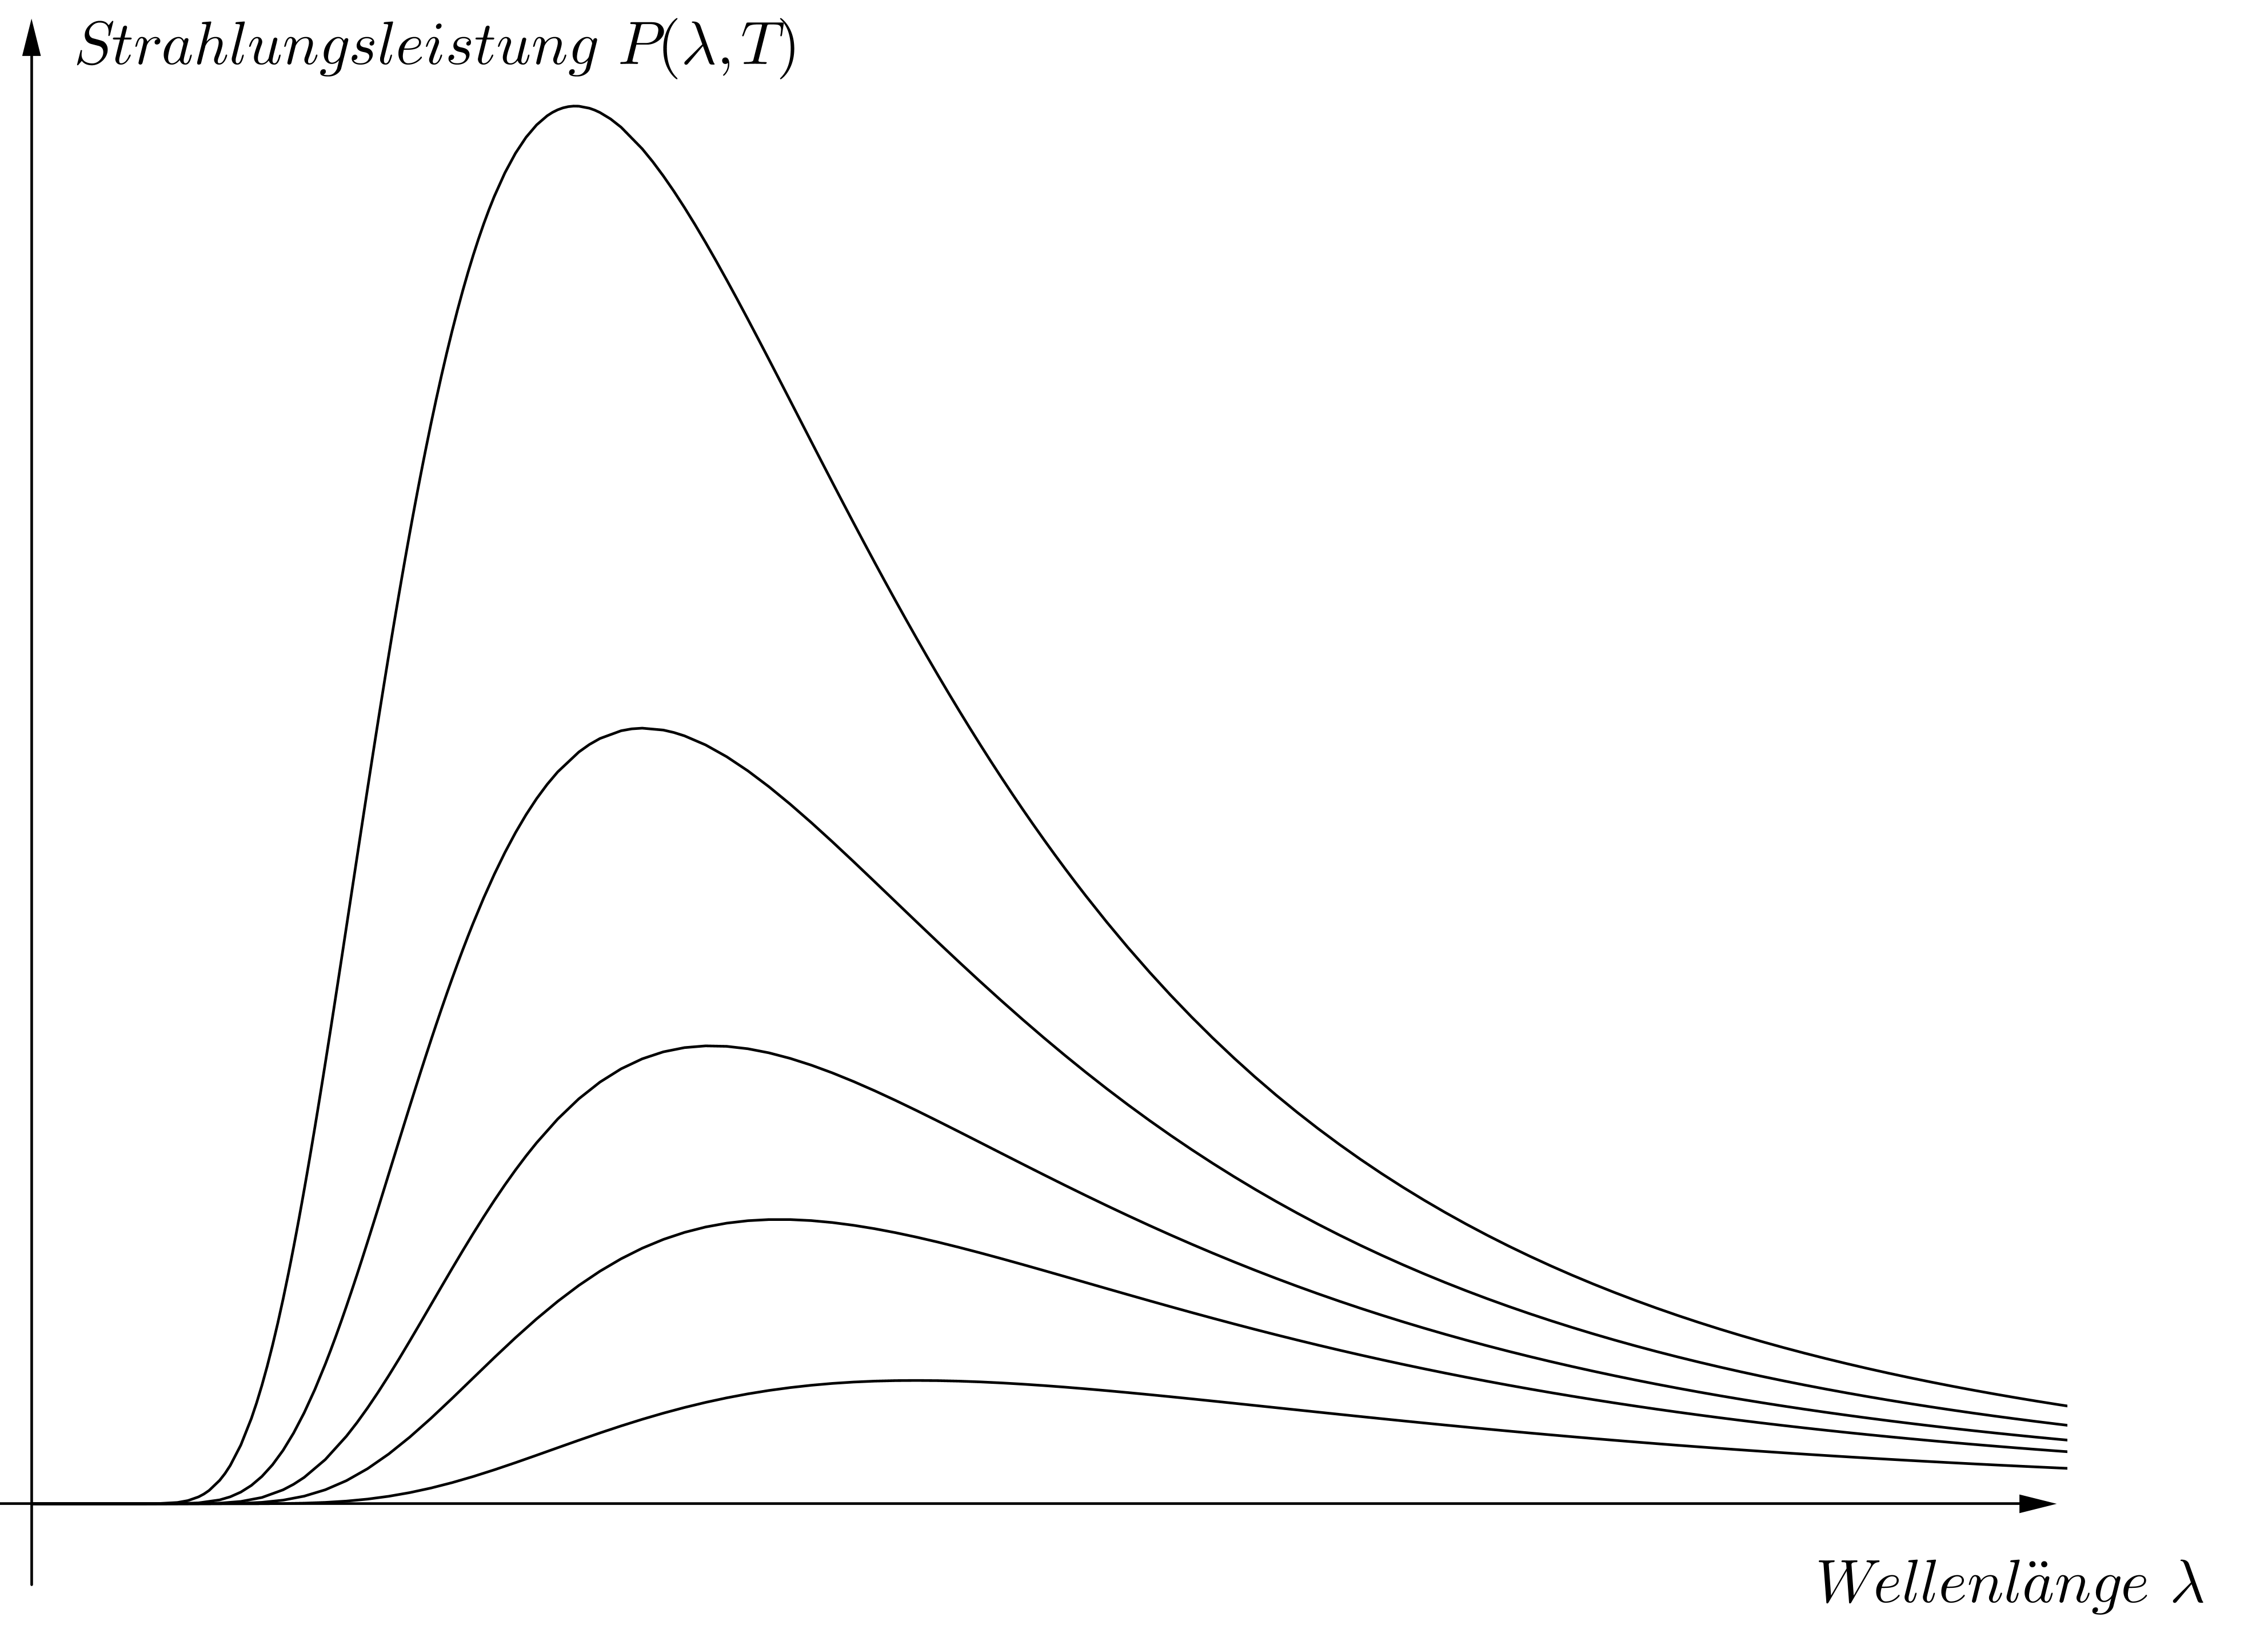
\includegraphics[width=0.75\textwidth]{pics/207a.png}
 \centering
 \caption{Plancksches Strahlungsspektrum zu verschiedenen Temperaturen}
 \label{Spektrum}
\end{figure}

Das in diesem Versuch zu untersuchende Stefan-Boltzmann-Gesetz beschreibt die Strahlungsdichte P(T) eines schwarzen Körpers und wird
dargestellt durch

\begin{formel}
\begin{equation}
 P(T) = \epsilon \, \sigma \, T^4
 \label{Boltz}
 \end{equation}
\caption*{\small{($\sigma$ = Stefan-Boltzmann-Konstante)}}
\end{formel}

\section{Durchführung}
Der Leslie-Würfel ist ein Würfel mit einer öffenbaren Deckelfläche mit einem Loch zur Temperaturmessung und vier verschiedenen Seitenflächen.
Eine schwarz lackierte, eine weiß lackierte, eine matt und eine glänzend metallische Fläche. Je nach Absorbtionsvermögen wird die Wärme
des Wassers aufgenommen und in Form von Wärmestrahlung wieder emittiert. Gemessen wird sie durch die Thermosäule nach Moll. Die eintretende
Strahlung von wird von in Reihe geschhalteten Thermoelementen erfasst, die thermisch mit dem Gehäuse verbunden sind. So wird eine relativ
zur Gehäusetemperatur T$_0$ ermittelte Temperatur angegeben. Der Wellenlängenbereich, für den die Thermosäule empfindlich ist, bewegt sich
zwischen $\lambda$ = 0,2 - 50 $\mu$m und mit Schutzfenster bei $\lambda$ = 0,3 - 2,8 $\mu$m.

\begin{figure}[H]
 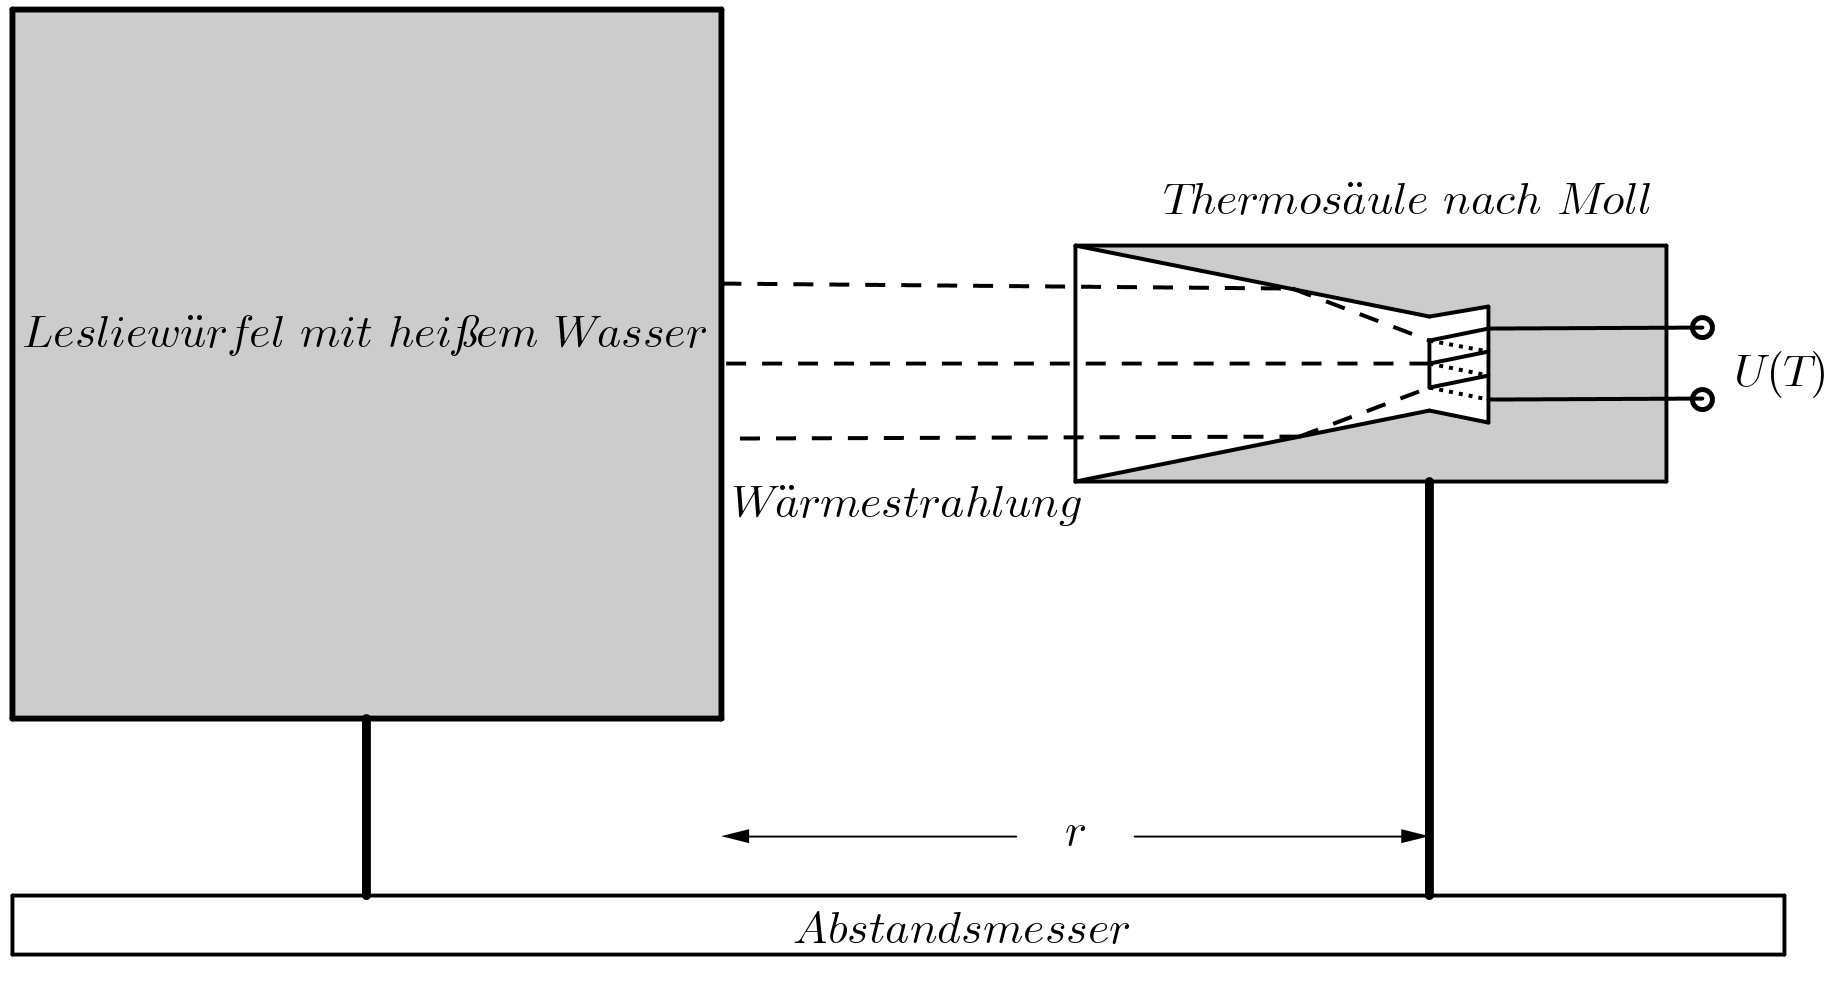
\includegraphics[width=0.9\textwidth]{pics/207b.png}
 \centering
 \caption{Schematischer Versuchsaufbau}
 \label{Aufbau}
\end{figure}

Nachdem ein Abstand von 10 cm zwischen der Thermosäule und der frontal gerichteten Würfelseitenfläche eingestellt worden ist, wird 
Wasser im Wasserkocher auf ungefähr 95 $^\circ$C erhitzt und in den Lesliewürfel gefüllt. Die Temperatur wird unterdessen permanent
gemessen. Über einen Zeitraum von $t$ = 5 min wird im Zeitintervall $\Delta t$ = 10 s die Thermospannung am Messgerät abgetragen. Das
nun für weitere Messungen zu kühle Wasser wird ausgeschüttet und durch neu erhitztes ersetzt. Ziel dieses Versuchsteils ist es, ausgehend
von 100 $^\circ$C im Temperaturintervall $\Delta T$ = 5 $^\circ$C die Thermospannung aller vier Seitenflächen zu messen und durch den
linearen Fit das Emissionsvermögen $\epsilon$ zu bestimmen. Die Offsetspannung, also jene Spannung, die die Temperatur der Luft
erzeugt, wird allenthalben vor und nach jeder Messung erfasst.

\section{Auswertung}
\subsection{Bestimmung der Ansprechzeit}
Zunächst soll die Ansprechzeit der Thermosäule bestimmt werden. Das ist die Zeit, die die Thermosäule benötigt, um die einfallende Wärme vollständig zu erfassen. Die Ansprechzeit ist daher für den weiteren Verlauf des Versuchs wichtig, denn man muss, nachdem man die Thermosäule auf eine andere Fläche des Würfels richtet, mindestens die Ansprechzeit abwarten, bevor Werte abgelesen werden dürfen.

Nachdem siedendes Wasser in den Würfel gefüllt wurde, wird die Thermospannung alle 10s abgelesen.

\begin{figure}{H}
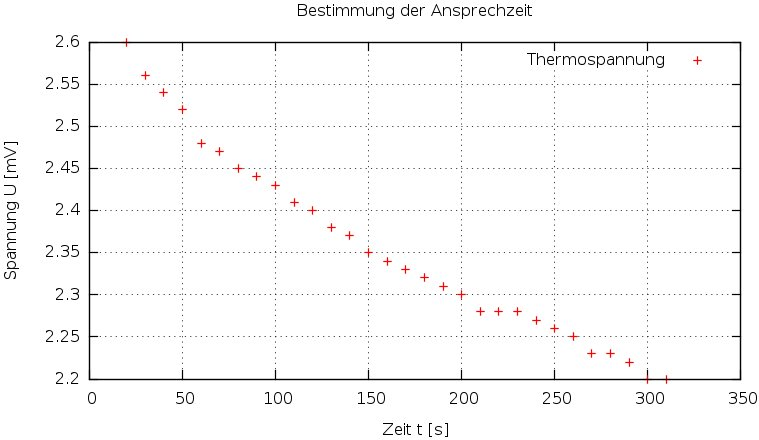
\includegraphics[width=0.9\textwidth]{pics/ansprechz.jpg}
\caption{Von der Thermosäule erzeugte Thermospannung gegen die Zeit aufgetragen}
\end{figure}

Gesucht wird nach einem Maximum des Graphens, da dies der Zeitpunkt ist, zu dem die Thermosäule die Wärme komplett anzeigt. Dieses lokale Maximum gibt es jedoch nicht, da die Spannung bereits innerhalb der ersten 5s ihren Endwert erreicht hat. Folglich ist bei den folgenden Messungen darauf zu achten, mindestens 5 Sekunden zu warten, bevor ein Wert abgelesen wird.
\begin{equation}
\text{Ansprechzeit }\approx 5[s]
\end{equation}

\subsection{Bestimmung des Emissionsvermögens $\epsilon$}
Um das Emissionsvermögen zu bestimmen wird der Würfel erneut mit siedendem Wassergefüllt und in jeweils $5^\circ$ Schritten die Thermospannung für alle 4 Würfelseiten notiert.

\begin{table}[H]
\begin{tabular}{|c|c|c|c|c|}
\hline 
Temperatur & Schimmernd [mV] & Schwarz [mV]& Matt [mV]& Weiß [mV]\\ 
\hline 
$82^\circ C$&-0.058	&1.842	&0.192	&1.802\\
\hline
$77^\circ C$&-0.078	&1.622	&0.132	&1.592\\
\hline
$72^\circ C$&0.612	&1.432	&0.082	&1.382\\
\hline
$67^\circ C$&-0.128	&1.232	&0.032	&1.202\\
\hline
$62^\circ C$&-0.137	&1.042	&0.002	&1.022\\
\hline
$57^\circ C$&-0.151	&0.852	&-0.030	&0.822\\
\hline
$52^\circ C$&-0.155	&0.672	&-0.058	&0.662\\
\hline
$47^\circ C$&-0.133	&0.530	&-0.068	&0.508\\ 
\hline
\end{tabular} 
\end{table}
Bei der schimmernden Oberfläche wurden die Werte bei $72^\circ C$ und $47^\circ C$ nicht in die Rechnung mit einbezogen, da sie zu stark von den anderen Abweichen. Möglicherweise hat sich das Gehäuse der Thermosäule zu diesen Zeitpunkten erwärmt, so dass die Messung verfälscht wurde.


\begin{figure}[H]
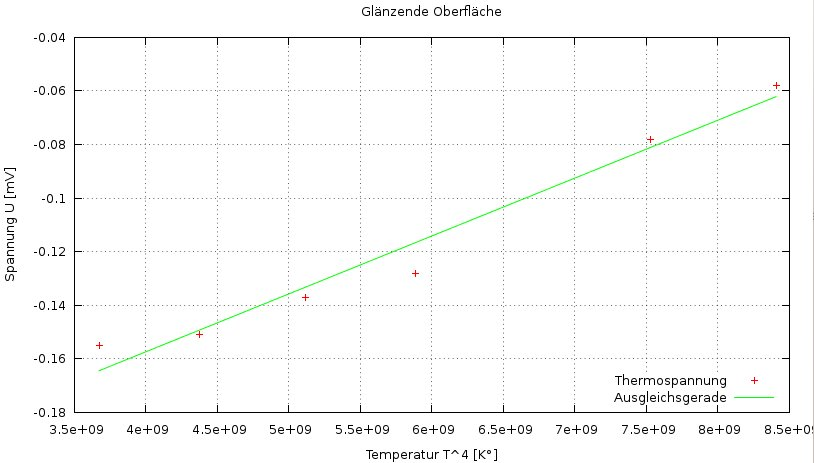
\includegraphics[width=0.9\textwidth]{pics/temp_schillernd.jpg}
\label{abstand}
\caption{Thermospannung an der schillernden Würfelseite}
\end{figure}

\begin{figure}[H]
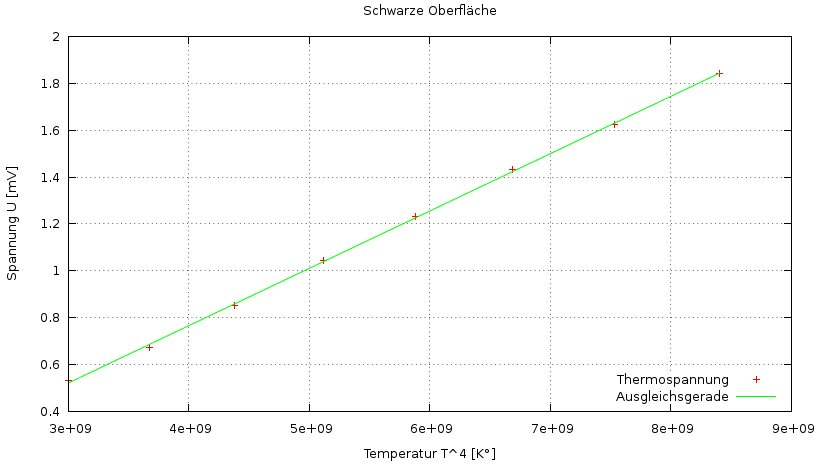
\includegraphics[width=0.9\textwidth]{pics/temp_schw.jpg}
\label{abstand}
\caption{Thermospannung an der schwarzen Würfelseite}
\end{figure}

\begin{figure}[H]
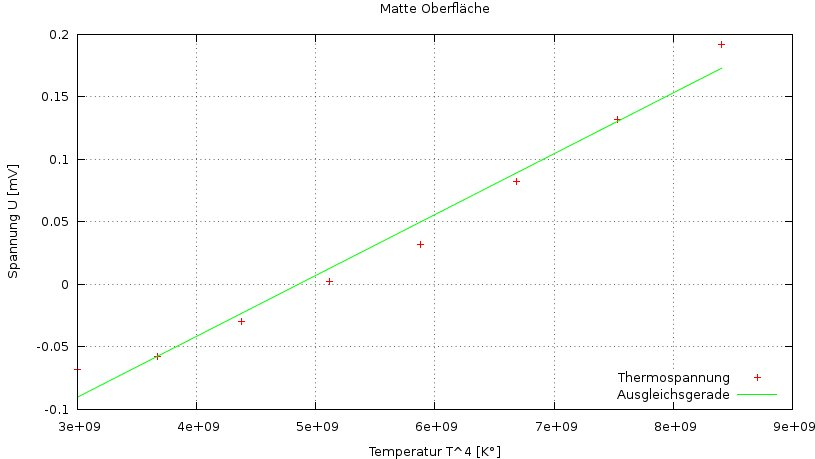
\includegraphics[width=0.9\textwidth]{pics/temp_matt.jpg}
\label{abstand}
\caption{Thermospannung an der matten Würfelseite}
\end{figure}

\begin{figure}[H]
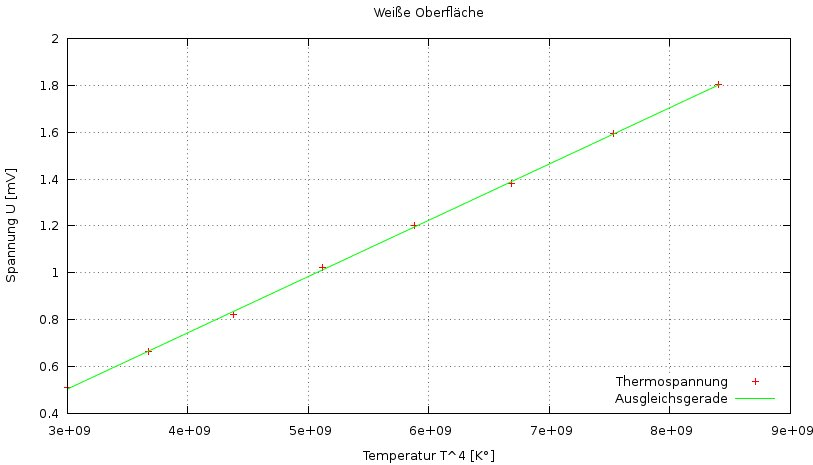
\includegraphics[width=0.9\textwidth]{pics/temp_weis.jpg}
\label{abstand}
\caption{Thermospannung an der weißen Würfelseite}
\end{figure}

Trägt man die gemessenen Spannungen gegen $T^4-T_0^4$ auf
\begin{align*}
\text{(mit } T_0=21,2^\circ C )
\end{align*}
und zeichnet eine Ausgleichsgerade ein, so hat diese nach Gleichung \eqref{Boltz} die Steigung $\epsilon\sigma$.

Nach einer Umrechnung der Daten der vier Oberflächen auf Volt errechnet man die Steigungen der Ausgleichsgeraden und dividiert diesen Wert nochmals durch $\sigma = 5,67\cdot 10^{-8}$ um das Emissionsvermögen $\sigma$ zu erhalten. 
\begin{align*}
\epsilon_{schillernd: }		&= 0,38\cdot10^{-6}     &\pm 0,04\cdot 10^{-6}  \\
\epsilon_{schwarz: }	 	&= 4,31\cdot10^{-6}     &\pm 0,03\cdot 10^{-6}  \\
\epsilon_{matt: }		 	&= 0,86\cdot10^{-6}     &\pm 0,05\cdot 10^{-6}  \\
\epsilon_{weiss: } 			&= 4,24\cdot10^{-6}     &\pm 0,03\cdot 10^{-6}  \\
\end{align*} 

Die schwarze Fläche soll nun als Schwarzer Strahler betrachtet werden. Dazu werden alle Werte so normiert, dass $\epsilon_{schwarz}=1$ ist.
Die Werte ändern sich dann zu:
\begin{align*}
\epsilon_{schillernd: }		&= 0,09      \\
\epsilon_{schwarz: }	 	&= 1         \\
\epsilon_{matt: }		 	&= 0,20      \\
\epsilon_{weiss: } 			&= 0,98      \\
\end{align*}
\subsection{Strahlintensität als Funktion des Abstandes}
Zum Schluss wird die Thermospannung für verschiedene Abstände von der schwarzen Würfelseite gemessen.

\begin{figure}[H]
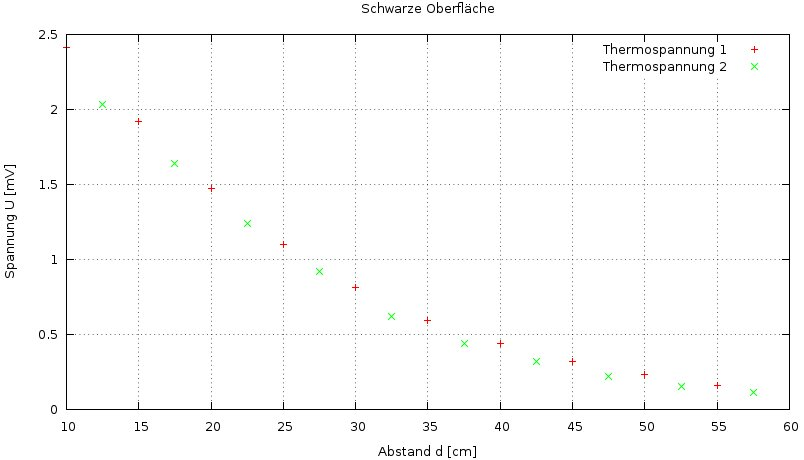
\includegraphics[width=0.9\textwidth]{pics/temp_abstand.jpg}
\caption{Thermospannung gegen den Abstand zum Würfel aufgetragen}
\label{abstand}
\end{figure}

Zur Erhöhung der Genauigkeit wurde im Abstand von etwa zwei Minuten eine zweite Messreihe aufgenommen. Da der Würfel in der Zwischenzeit etwas ausgekühlt ist, werden die Messreihen farbig unterschieden.

\section{Diskussion}
Das Emissionsvermögen der vier Seiten ist äußerst gering. Entsprechend hoch sind die Abweichungen einzelner Werte wegen Temperaturschwankungen der Umgebungstemperatur. Nach einer Normierung der Werte auf die schwarze Fläche, die als schwarzer Strahler betrachtet werden soll, ergeben sich Werte in einer Größenordnung, die zu erwarten waren. Interessant dabei ist, dass die weiße und die schwarze Fläche sehr ähnliche Werte haben. Es ist also unerheblich welche Farbe die Oberfläche hat, es kommt mehr auf die beschaffenheit des Materials an. Die metallenen Flächen haben die Wärme deutlich schlechter abgegeben als die mit Farbe bestrichenen. Insgesamt kam jedoch keine der Flächen einem schwarzen Strahler nah, da die unnormierten $\epsilon \ll 1$ sind.

Die Abgestrahlte Leistung nimmt wie zu erwarten mit dem Abstand vom Würfel ab. Die bestrahlte Fläche nimmt bei gleichbleibendem Raumwinkel mit $R^2$ zu, so dass die Strahlungsintensität an der Thermosäule mit $\frac{1}{R^2}$ abnimmt. Die aufgetragenen Werte im Graphen \eqref{abstand} belegen dies, da sie nahezu perfekt auf der $\frac{1}{R^2}$ Ausgleichsfunktion liegen.



% ========================================
%	Literaturverzeichnis
% ========================================

%\bibliographystyle{plainnat}			% Bibliographie-Style auswählen
%\bibliography{BIBDATEI}			% Literaturverzeichnis

% ========================================
%	Das Dokument endent
% ========================================

\end{document}
